% !TEX program = Xelatex
\documentclass{article}
\usepackage{amsmath,amscd,amsbsy,amssymb,latexsym,url,bm,amsthm}
\usepackage{epsfig,graphicx,subfigure}
\usepackage{enumitem,balance,mathtools}
\usepackage{wrapfig}
\usepackage{mathrsfs, euscript}
\usepackage{hyperref}
\usepackage{listings}
% \usepackage[ruled,lined,boxed,linesnumbered]{algorithm2e}
\usepackage[ruled]{algorithm2e}
\usepackage{tikz-network}
\usepackage{xcolor}
\usepackage{listings}
\lstset{
    basicstyle=\ttfamily,
    showstringspaces=false,
    commentstyle=\it\color[RGB]{0,96,96},
    keywordstyle=\color[RGB]{40,40,255},
    frame=lines,
    captionpos=b
}

% \hypersetup{hidelinks}

\newtheorem{theorem}{Theorem}[section]
\newtheorem{lemma}[theorem]{Lemma}
\newtheorem{proposition}[theorem]{Proposition}
\newtheorem{corollary}[theorem]{Corollary}
\newtheorem{exercise}{Exercise}[section]
\newtheorem*{solution}{Solution}

\renewcommand{\thefootnote}{\fnsymbol{footnote}}
\newcommand{\postscript}[2]
    {\setlength{\epsfxsize}{#2\hsize}
    \centerline{\epsfbox{#1}}}
\renewcommand{\baselinestretch}{1.0}

\setlength{\oddsidemargin}{-0.365in}
\setlength{\evensidemargin}{-0.365in}
\setlength{\topmargin}{-0.3in}
\setlength{\headheight}{0in}
\setlength{\headsep}{0in}
\setlength{\textheight}{9.1in}
\setlength{\textwidth}{7in}

% ------ adjust it according to the specific circumstances ----- %
\title{EI338 Computer Systems Engineering}
\author{Project 1}
% \date{}
% ---------------------------------------------------------------%

\begin{document}

\maketitle

% ------------------ your name and number ----------------- %
\begin{center}
    Zhihui Xie, 517030910356
\end{center}

% --------------------------------------------------------- %
The environment used in this project is \textbf{Deepin 15.11}, the latest version of an open source operating system based on Debian's stable branch. The kernel version is \textbf{Linux version 4.15.0}.

\section*{Exercise 1}
    \subsection*{Question}
    Design a kernel module that creates a \textit{/proc} file named \textit{/proc/jiffies}
    that reports the current value of \textbf{jiffies} when the \textit{/proc/jiffies} file
    is read, such as with the command

    \vspace{2pt}

    \begin{lstlisting}[language=bash]
cat /proc/jiffies
    \end{lstlisting}

    \vspace{2pt}

    Be sure to remove \textit{/proc/jiffies} when the module is removed.
        
    \subsection*{Thinking} It would not be a problem reporting the value of \textbf{jiffies} since it is directly declared in \textit{<linux/jiffies.h>}. The difficulty may lies in the understanding of each part of kernel structure in our first attempt of kernel designing. 
    
    \subsection*{Answer} In this exercise, we design a kernel module named \textit{jiffies}. There are mainly three parts or three functions to realize our purpose.
    \begin{enumerate}
        \item[-] \textbf{proc\_init()}, the module entry point 
        \item[-] \textbf{proc\_exit()}, the module exit point
        \item[-] \textbf{proc\_read()}, the function called when the specific \textit{/proc} file is read  
    \end{enumerate}

    \subsubsection*{proc\_init()}
    In \textbf{proc\_init()}, we create the new \textit{/proc/jiffies} entry using the \textbf{proc\_create()} function. This function is passed \textbf{proc\_ops} which contains a reference to a struct \textbf{file\_operations}. It serves as a simple interface to create the \textit{/proc} file system. This struct initializes the \textbf{.owner} and \textbf{.read} members. The value of \textbf{.read} is the name of the function \textbf{proc\_read()}. An message is sent to a kernel log buffer using \textbf{printk()} to notice that the module is successfully inserted.

    \vspace{2pt}

    \begin{lstlisting}[language=c, caption={\textbf{proc\_init()}}]
/**
* Function prototypes
*/
static ssize_t proc_read(struct file *file, char *buf, size_t count, loff_t *pos);

static struct file_operations proc_ops = {
        .owner = THIS_MODULE,
        .read = proc_read,
};

/* This function is called when the module is loaded. */
static int proc_init(void)
{

        // creates the /proc/jiffies entry
        // the following function call is a wrapper for
        // proc_create_data() passing NULL as the last argument
        proc_create(PROC_NAME, 0, NULL, &proc_ops);

        printk(KERN_INFO "/proc/%s created\n", PROC_NAME);

    return 0;
}
    \end{lstlisting}

    \vspace{2pt}

    \subsubsection*{proc\_exit()}
    In \textbf{proc\_exit()}, we need to remove the \textit{/proc/jiffies} using the function \textbf{remove\_proc\_entry()}. An message is sent to a kernel log buffer using \textbf{printk()} to notice that the module is successfully removed.

    \vspace{2pt}

    \begin{lstlisting}[language=c, caption={\textbf{proc\_exit()}}]
static void proc_exit(void) {

        // removes the /proc/jiffies entry
        remove_proc_entry(PROC_NAME, NULL);

        printk( KERN_INFO "/proc/%s removed\n", PROC_NAME);
}
    \end{lstlisting}

    \vspace{2pt}

    \subsubsection*{proc\_read()}
    In \textbf{proc\_read()}, we are dealing with how to report the current value of \textbf{jiffies} when the \textit{/proc/jiffies} file is read. It is not a big deal to get the value of \textbf{jiffies} since it is directly declared in the file \textit{<linux/jiffies.h>}. The real problem is about how can we display it in the command line. 

    The read handler \textbf{proc\_read()} receives 4 parameters:

    \begin{enumerate}
        \item[-] File object \textbf{*file}, per process structure with the opened file details (permission , position, etc.)
        \item[-] User space buffer \textbf{*usr\_buf}
        \item[-] Buffer size \textbf{count}
        \item[-] Requested position \textbf{*pos}
    \end{enumerate}

    To implement the read callback, we need to:

    \begin{enumerate}
        \item[-] Check the requested position
        \item[-] Fill the user buffer with a data (max size $\leq$ buffer size) from the requested position
        \item[-] Return the number of bytes we filled
    \end{enumerate}

    We first check if it is the first time we read the file and the user buffer size is bigger than \textbf{BUFFER\_SIZE}. If not, we return 0 to indicate that there is nothing to read. Finally, we build the returned buffer, copy it to the user, update the position and return the number of bytes we wrote. And it is worth mentioning why we use the function \textbf{copy\_to\_user()}. We use it to memcpy the data from the user space to the kernel space since it is not accessible for us to directly deal with the buffer in kernel space. 

    \vspace{2pt}

    \begin{lstlisting}[language=c, caption={\textbf{proc\_read()}}]
static ssize_t proc_read
(struct file *file, char __user *usr_buf, size_t count, loff_t *pos)
{
        char buffer[BUFFER_SIZE];
        int len = 0;

        if(*pos > 0 || count < BUFFER_SIZE) return 0;
            
        len += sprintf(buffer, "The total number of interrupts is %lu\n", jiffies);

        // copies the contents of buffer to userspace usr_buf
        copy_to_user(usr_buf, buffer, len);

        // updates the position and returns the number of bytes we received
        *pos = len;
        return len;
}
    \end{lstlisting}

    \vspace{2pt}

    Each time the \textit{/proc/jiffies} file is read, the \textbf{proc\_read()} function is called repeatedly until it returns 0.

    \subsection*{Experiment}
    We directly present the commands in shell.

    \begin{figure}[h]
        \centering
        
        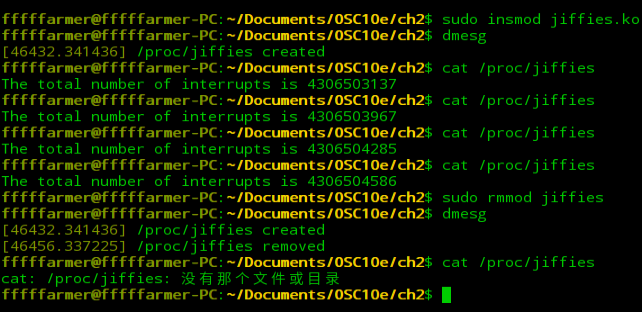
\includegraphics[width=17cm]{jiffies}
        \caption{Experiment Result in Exercise 1}
        \label{}
    \end{figure}

    \section*{Exercise 2}
    \subsection*{Question}
    Design a kernel module that creates a \textit{proc} file named \textit{/proc/seconds}
    that reports the number of elapsed seconds since the kernel module was loaded. This will involve using the value of \textbf{jiffies} as well as the \textbf{HZ}
    rate. When a user enters the command

    \begin{lstlisting}[language=bash]
cat /proc/seconds
    \end{lstlisting}

    your kernel module will report the number of seconds that have elapsed since the kernel module was first loaded. Be sure to remove \textbf{/proc/seconds} when the module is removed.
    
    \subsection*{Thinking} This time, we need to keep some value. We may use a global variable to address this. Nothing new.
    
    \subsection*{Answer}
    All three main functions are realized in a way similar to that in Exercise 1. The main difference lies on the output: the output changes depending on when we call the function. Besides this, everything is the same. 

    To address this, we declare a global variable named \textbf{interrupt\_start} to record the value of \textbf{jiffies} when the module is loaded. 

    And in \textbf{proc\_init()}, we assign the current value of \textbf{jiffies} to it. 

    \vspace{2pt}

    \begin{lstlisting}[language=c, caption={\textbf{proc\_init()}}]
static int proc_init(void)
{
        
        // ...

        interrupt_start = jiffies;
	return 0;
}
    \end{lstlisting}

    \vspace{2pt}

    The function \textbf{proc\_exit()} keeps the same. In \textbf{proc\_read()}, we need to simply calculate the elapsed seconds using \textbf{HZ} and the difference between current \textbf{jiffies} and \textbf{interrupt\_start}.

    \vspace{2pt}

    \begin{lstlisting}[language=c, caption={\textbf{proc\_read()}}]
static ssize_t proc_read
(struct file *file, char __user *usr_buf, size_t count, loff_t *pos)
{
        // ...

        unsigned long int interrupts = jiffies - interrupt_start;

        // ...

        len += sprintf(buffer, "The number of elapsed seconds 
        since the kernel module was loaded is %lus\n", interrupts/HZ);

        // ...

	return len;
}
    \end{lstlisting}

    \subsection*{Experiment}
    We directly present the commands in shell. To show that our output is correct, we check the system time as reference.

    \begin{figure}[h]
        \centering
        
        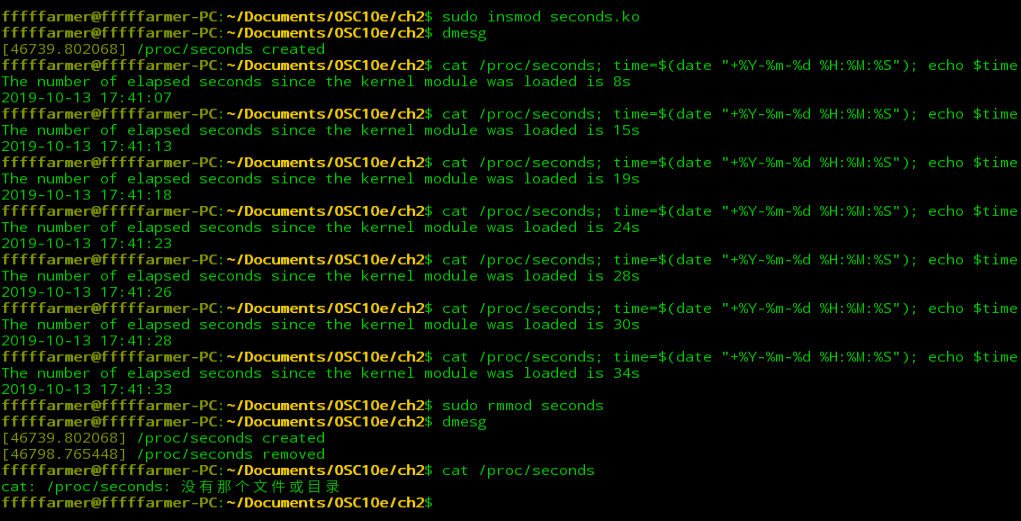
\includegraphics[width=17cm]{seconds}
        \caption{Experiment Result in Exercise 2}
        \label{}
    \end{figure}


\end{document}